\documentclass[12pt]{article}

\usepackage[english]{babel}
\usepackage[utf8x]{inputenc}
\usepackage{pdfpages}
\usepackage{lastpage} % Required to determine the last page for the footer
\usepackage{extramarks} % Required for headers and footers
\usepackage{graphicx} % Required to insert images
\usepackage{listings} % Required for insertion of code
\usepackage{courier} % Required for the courier font
\usepackage{color}
\usepackage{grffile}
\usepackage{float}

\usepackage[a4paper, total={6in, 8in}]{geometry}

% Margins
\topmargin=-0.45in
\evensidemargin=0in
\oddsidemargin=0in
\textwidth=6.5in
\textheight=9.0in
\headsep=0.25in
\fboxsep=0mm%padding thickness
\fboxrule=2pt%border thickness

\linespread{1.1} % Line spacing

\newcommand{\Title}{Vision and scope document} % Assignment title
\newcommand{\Class}{COS\ 301 Final year project} % Course/class
\newcommand{\pd}{Post-Doctoral}
\newcommand{\ssr}{Soft\color{green}{Serve }\color{black}}
\newcommand{\version}{3.0 (Final)}
\newcommand{\iteration}{6}
\newcommand{\client}{Ms. Cathy Sandis (UP DRIS)}
\newcommand{\supervisor}{Prof. Stefan Gruner (SSFM Group)}
\newcommand{\project}{Post-Doctoral management System}
\newcommand{\repo}{https://github.com/mox1990/Project-Postdoc.git}

\begin{document}


\vspace{4em}

\begin{center}%

\begin{figure}[ht!]
\centering

\includegraphics{../Images_Docs/logo.png}
\end{figure}
\LARGE \bf \Class \\[0.25em]
\LARGE \bf \project \\[1em]
\LARGE \bf \Title \\[0.25em]
\large \bf \today\\
\bf Version \version\\
\bf Iteration \iteration\\[0.5em]
\Large \bf Prepared for \\Client: \client\\Supervisor: \supervisor
\Large \\\bf by \\
\Large {\bf \ssr Group }\\[0.5em]
\LARGE {\bf Group members}\\[0.25em]
\large
Kgothatso Phatedi Alfred Ngako (12236731) \\[0.5em]
Tokologo “Carlo” Machaba (12078027) \\[0.5em]
Mathys Ellis (12019837) \\[8em]

\end{center}%

%\newpage
%{\LARGE \bf Change log}\\[2em]

\begin{center}
\begin{tabular}{|l|p{1.4cm}|p{8cm}|p{2.8cm}|}
\hline
\multicolumn{4}{|c|}{\bf Change log} \\
\hline
 Date & Version & Description &  Person \\
\hline
10/02/2014 & v 0.0 & Original SRS document created. & Mathys Ellis \\
\hline
02/03/2014 & v 0.1 & Added to glossary. & Mathys Ellis \\
\hline
05/03/2014 & v 0.3 & Added Introduction, Vision, Background. & Carlo Machaba \\
\hline
06/03/2014 & v 0.4 & Added open issues. Modified some sections. & Alfred Ngako \\
\hline
06/03/2014 & v 0.5 & Added methodology, scope and limitations. & Mathys Ellis \\
\hline
08/03/2014 & v 0.6 & Added some wrapping to the change log which is now a table. & Alfred Ngako \\
\hline
16/03/2014 & v 0.8 & Did some restructuring and document formatting. & Mathys Ellis \\
\hline
17/03/2014 & v 0.8 & Also added to the glossary. & Mathys Ellis \\
\hline
12/05/2014 & v 0.9 & Created new vision and scope document. Transferred necessary content from old SRS document. Performed editing and restructuring of document. Added exclusions. & Mathys Ellis \\
\hline
16/05/2014 & v 0.95 & Updated use case diagrams and stakeholders. & Mathys Ellis \\
\hline
21/05/2014 & v 1.0 & Added import and export services and application process. Finalised document for first iteration. & Mathys Ellis \\
\hline
01/10/2014 & v 2.0 & Added, refined and reordered document to meet new demands. & Mathys Ellis \\
\hline
17/10/2014 & v 3.0 & Finalised and revised document & Mathys Ellis \\
\hline

\end{tabular}
\end{center}
\newpage
\tableofcontents

\listoffigures
\newpage
\section{Project Repository}
\textbf{\repo}
\newpage
\section{Document description:}

\subsection{Document purpose:}
\vspace{0.2in}
This vision and scope document serves the purpose of providing a detailed overview of the project's scope and its vision as well the goals that SoftServe's Post-Doctoral management system wishes to satisfy. Further it defines the abstract interaction of stakeholders with the proposed software system. Thus this document serves as a contract between SoftServe and the client, Mrs Cathy Sandis of the DRIS of the University of Pretoria in terms of project scope.

\vspace{0.2in}

\subsection{Documentation methodology}
\vspace{0.2in}
\begin{flushleft}
The documentation and software development methodology used by the project adhere to the guidelines set out by the scrum agile methodology. Thus this document has undergone and will undergo various iterations that may extend or reduce the contents of the document.\\

This document was created using the requirement elicitation techniques and requirement definitions as specified by Klaus Pohl’s book Requirements Engineering: Fundamentals, Principles, and Techniques [Dr.Phol, K., 2010].
The requirements, vision and scope were elicited from the following sources:
\begin{itemize}
	\item Numerous interviews with the client.
	\item On-line research into UP Post doctoral applications.
	\item Correspondence with the UP IT department.
	\item Collecting and analysing various documents such as:
		\begin{itemize}
			\item The initial project request document
			\item Application forms
			\item Renewal forms
			\item CV templates
			\item Approval and recommendation forms
		\end{itemize}
\end{itemize}
\end{flushleft}	

\vspace{0.5in}

\subsection{Document conventions:}
\vspace{0.1in}
\begin{itemize}
\item Documentation formulation tool: LaTeX
\item Modelling language: UML 2.0
\end{itemize}

\vspace{0.2in}

\subsection{References:}
\vspace{0.1in}
\begin{itemize}
\item Dr.Phol, K., 2010, \textit{Requirements Engineering: Fundamentals, Principles, and Techniques}, Springer, Heidelberg.
\item DRIS homepage. [online] Available: \textit{http://web.up.ac.za/default.asp?ipkCategoryID=1630} [Accessed on: 31 March 2014].
\end{itemize}	

\vspace{0.5in}

\newpage
\section{Project introduction}
A Post-Doctoral fellow is a person who conducts research after they have completed their PhD, with the aim of deepening their knowledge in a specific field. The University of Pretoria, UP, supports such research opportunities in order to increase the research output of UP itself. Post-Doctoral fellows who conduct their research at UP do so under the supervision of a appropriate academic staff member at the University and their research may be externally or internally funded. This is a growing field in Universities around South Africa. A lack in the software solutions for the application management of Post-Doctoral fellows has been identified by the SoftServe group. To exploit this opportunity the SoftServe group has proposed the following project.
 
\vspace{0.2in}

\section{Project background}
\vspace{0.2in}
The current Post-Doctoral prospective and renewal application processes are paper based thus there are a number of drawbacks, mainly due to human error. One such drawback is that there is no audit trail when it comes to the input of the different stakeholders involved in approving or declining the applications. Another involves the minutes of Post-Doctoral committee meetings which are often misplaced or typed in an inconsistent manner making it hard to recall what has been discussed in such meetings. These meetings play a critical part in the evaluation of prospective and renewal applications thus this is an area of concern. Access to the documents involved in the application process is also a problem since they are usually hard copies that change hands constantly. Thus the process of getting access to the documents is long and tedious if not made impossible, since they run the risk of being lost due to various factors. Reporting on the information of fellows, applications, renewals, etc, as well as even communication with the different stakeholders is also problematic due the current system not begin centralised and changing nature of the academics structure in UP. Therefore gathering all the information required to generate accurate reports is difficult or even impossible. Another factor is the complexity of workflow makes it diffuclty to maintain it on the current paper-basis. Also this makes it difficult to train new DRIS administrators for the processes. These problems lead the client, Mrs Cathy Sandis, to see a potential area that could be optimised by the implementation of a digitalised system. At this point the SoftServe group was brought into the picture.
\vspace{0.5in}

\newpage
\section{Project vision}
\vspace{0.2in}
The client needs a system which can make the management of the prospective and renewal application processes of Post-Doctoral fellowships, from start to end, more effective, intractable, reliable, secure and audit-able. And also provide the necessary auxiliary services to support the application process and make use of its data. Together the client and SoftServe have envisioned a system that will make use of a centralised user friendly web interface that will be used by the all the stakeholders involved in the various processes. The system will host various sections that handle the different stages in the work-flow of the processes. The system will need to automate the transitions between stages by forwarding the required information to the next stakeholder in the process and notifying them via an email notification or equivalent. The system will also need to provide reporting facilities for the application and person information stored by the system. As well as progress tracking with regards to any application. The system data needs to be centralised to ensure that any information used by system is cohesive and valid for any stakeholder who accesses it. Another feature the system should host is that of archival support so that old data can be retrieved if needed and also backup support. The system will also need to allow for the recreation of existing data with regards to applications, people and locations, which act as importing facilities. The work-flow of applications is not a very dynamic but has been known to change from time to time therefore some kind of simple mechanism needs to be implemented by the system in order to improve maintainability of the work-flow. Further the system will be standalone but might need to integrate with other software solutions hosted by UP or external systems thus it should be made integrate-able via standardisation and APIs. By introducing a digital system, as described above, the client hopes that the management of Post-Doctoral fellows will be easier to track and manage.
\vspace{0.5in}

\newpage
\section{Stakeholders}

The stakeholders that will engage or be engaged by the system are listed below:

There are four categories under which stockholders can fall:
\begin{itemize}	
\item System or abstract:
These are stakeholders that represent the system itself and generalized users based on their security roles:
\begin{itemize}
\item \textbf{System} - The actual Post-Doctoral management system.
\item \textbf{System administrator} - The super user of the Post-Doctoral management system. This user has universal access.
\item \textbf{Authorised user} - A user that has the necessary security roles to perform the operation.
\end{itemize}
\item External individuals:
These are stakeholders that do not have a PeopleSoft account or are prospective fellows.
\begin{itemize}	
\item \textbf{Prospective fellow} - A person who wishes to apply for a post-doctoral research fellowship.
\item \textbf{Referee} - A person who is identified by a Prospective fellow as a referral.
\end{itemize}

\item Internal individuals:
These are stakeholders that do have a PeopleSoft account and are individual members of staff.
\begin{itemize}	
\item \textbf{Research fellow} - A person who is currently in possession of a fellowship.
\item \textbf{Grant holder} - The person who is a fellow's supervisor and a academic member of staff at the University of Pretoria. This person is also known as the applicant.
\item \textbf{HOD} - The head of a department at UP. Note that this may also be the Grant holder of some applications.
\end{itemize}
\item Internal groups:
These are stakeholders that do have a PeopleSoft account and are a group of staff members.
\begin{itemize}	
\item \textbf{Dean's office} - The dean and deputy dean of a faculty at UP. Thus they oversee the various departments which fall underneath them. In some cases this may be the dean and deputy dean of research for that faculty if the faculty provides such a responsibility.
\item \textbf{DRIS} - The department of Research and Innovation Support at the University of Pretoria. This stakeholder oversees the processes and utilises the system for administrative tasks.
\item \textbf{Post-doctoral committee} - This is a committee who reviews and evaluates any post-doctoral fellowship applications.
\item \textbf{CSC} - The client service centre of the University of Pretoria. Note this stakeholder has no direct access to the system rather the system provides means only a means to forward information to them.
\item \textbf{Finance} - The department of finance at the University of Pretoria. Note this stakeholder has no direct access to the system rather the system provides only a means to forward information to them.
\end{itemize}
\end{itemize}
\vspace{0.5in}

\newpage
\section{Project Scope:}
\vspace{0.2in}

\subsection{System scope}
	
The scope of the project is to design a Post-Doctoral management system in the form of a software package where prospective fellows can apply for fellowships and current Post-Doctoral research fellows can renew their fellowships at the University of Pretoria. The system will manage the application work-flow from the start until the end of the process. Where the end is defined as follows: When the DIRS have either terminated or closed the application, or if the fellowship has been completed or when the application has been denied approval. Further the system will also incorporate non-application services to support and enhance both the administration of the system and application work-flow. As well provide means to extract and use information from the data stored by the system. The system will also be designed so to allow for future integration with the current student and personnel management system, PeopleSoft, employed by the UP. As well as any other possible system by providing the necessary APIs and mechanisms to do so. Finally the proposed system will be a stand-alone system.
\vspace{0.2in}

\newpage
\subsubsection{Use cases:}
This section shows the use cases for the entire system. For a more  detailed view of each use cases please refer to the Functional requirements and application design document for the project 
\begin{figure}[H]
\centering	
\framebox{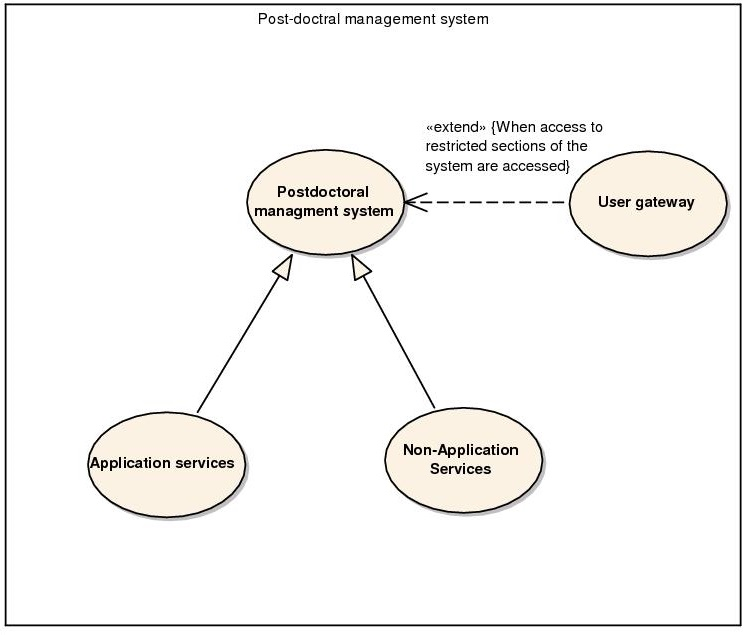
\includegraphics[scale=0.8]{../Images_Docs/Diagrams/Use case diagrams/Post-doctral fellowship management system1.jpg}}
\caption{Use case diagram of Post-doctoral management system}
\end{figure}

\newpage
\subsection{Application services scope}
This section discusses and gives an abstract overview of the post-doctoral prospective and renewal application processes. Each of the processes are broken up in stages. Each of the stage needs to be passed for the application to proceed to the next. It should be noted that the client has pointed out that sometimes a stage or several stages have not been completed by the application though at the discretion of the DRIS the application may be pushed forward to the required stage. The stages are numbered in accordance to the order in which they occur. It should be noted that both processes only differ at the second stage and slightly at other stages and that the renewal process is a extension of the prospective application process.

\begin{itemize}
	\item New application
		\begin{enumerate}
			\item A prospective fellow opens a application for a post-doctoral fellowship.
			\item If the application is a UP Postdoc application it requires that at least 2 referees are specified by the prospective fellow, each have to complete a referral report. The grant holder is also notified once all the referral reports are completed. 
			\item The identified grant holder has to communicate with the prospective fellow in order to verify and finalise the application once all the referral reports are acquired if there are. If the grant holder is not satisfied then they can ask for amendment. The grant holder may deny the application if they feel so. The prospective fellow is also notified of this. 
			\item The finalised application is then given to HOD of the specified department for approval. On approval the application is supplemented with a recommendation report. The HOD can ask for amendment if he/she feels the need or even deny the application.
			\item The application is then given to the appropriate member of the dean's office who then needs to approve it. On approval the application needs to be endorsed by a motivational letter and rank order based on score out of 10. The dean's office may deny the application. The prospective fellow and grant holder is also notified of this. 
			\item The endorsed application is given to the appropriate member of the DRIS for eligibility checking. If found eligible the application is moved to the next stage. Else it is denied. The prospective fellow and grant holder is also notified of this. 
			\item The DRIS member has to arrange and convene a post-doctoral meeting after the application deadline of the eligible applications. This documentation is the collection of all the related application data that has been added to the application at each stage. The prospective fellow and grant holder is also notified of this. 
			\item The post-doctoral meeting is then convened where the members of the post-doctoral committee evaluate and deliver their insights into the potential applications. This is documented in the form of minute meetings. 
			\item The appropriate member(s) of the DRIS then need to make the final funding decision of all the applications based on the minute meetings and record this data. They can approve it or decline the application. If approved they need to add the final application information as well as the funding information.
			\item The data is then summarised accordingly and sent to the finance department as well as the CSC. The prospective fellow and grant holder is also notified of this.   
		\end{enumerate}
	\item Renewal application
		\begin{enumerate}
			\item A research fellow opens a renewal application for a post-doctoral fellowship.
			\item The research fellow then needs to complete a final progress report if they have not yet done so.
			\item The identified grant holder has to communicate with the prospective fellow in order to verify and finalise the renewal application once the renewal is submitted by the fellow. If the grant holder is not satisfied then they can ask for amendment. The grant holder may deny the application if they feel so. The research fellow is notified of this.  
			\item The finalised application is then given to HOD of the specified department for approval. On approval the application is supplemented with a recommendation report. The HOD can ask for amendment if he/she feels the need or even deny the application. The research fellow and grant holder is also notified of this.  
			\item The application is then given to the appropriate member of the dean's office who then needs to approve it. On approval the application needs to be endorsed by a motivational letter and rank order based on score out of 10. The dean's office may deny the application. The research fellow and grant holder is also notified of this.  
			\item The endorsed application is given to the appropriate member of the DRIS for eligibility checking. If found eligible the application is stored. Else it is denied. The research fellow and grant holder is also notified of this.  
			\item The DRIS member has to arrange and convene a post-doctoral meeting after the application deadline and prepare the pre-documentation of the eligible applications. This documentation is the collection of all the related application data that has been added to each of the initial applications.
			\item The post-doctoral meeting is then convened where the members of the post-doctoral committee evaluate and deliver their insights into the potential applications. This is documented in the form of minute meetings. 
			\item The appropriate member(s) of the DRIS then need to make the final funding decision of all the applications based on the minute meetings and record this data. They can approve it or decline the application. If approved they need to add the final application information as well as the funding information.
			\item The data is then summarised accordingly and sent to the finance department as well as the CSC. The research fellow and grant holder is also notified of this.    
		\end{enumerate}

	
\end{itemize}

\begin{figure}[H]
\centering	
\framebox{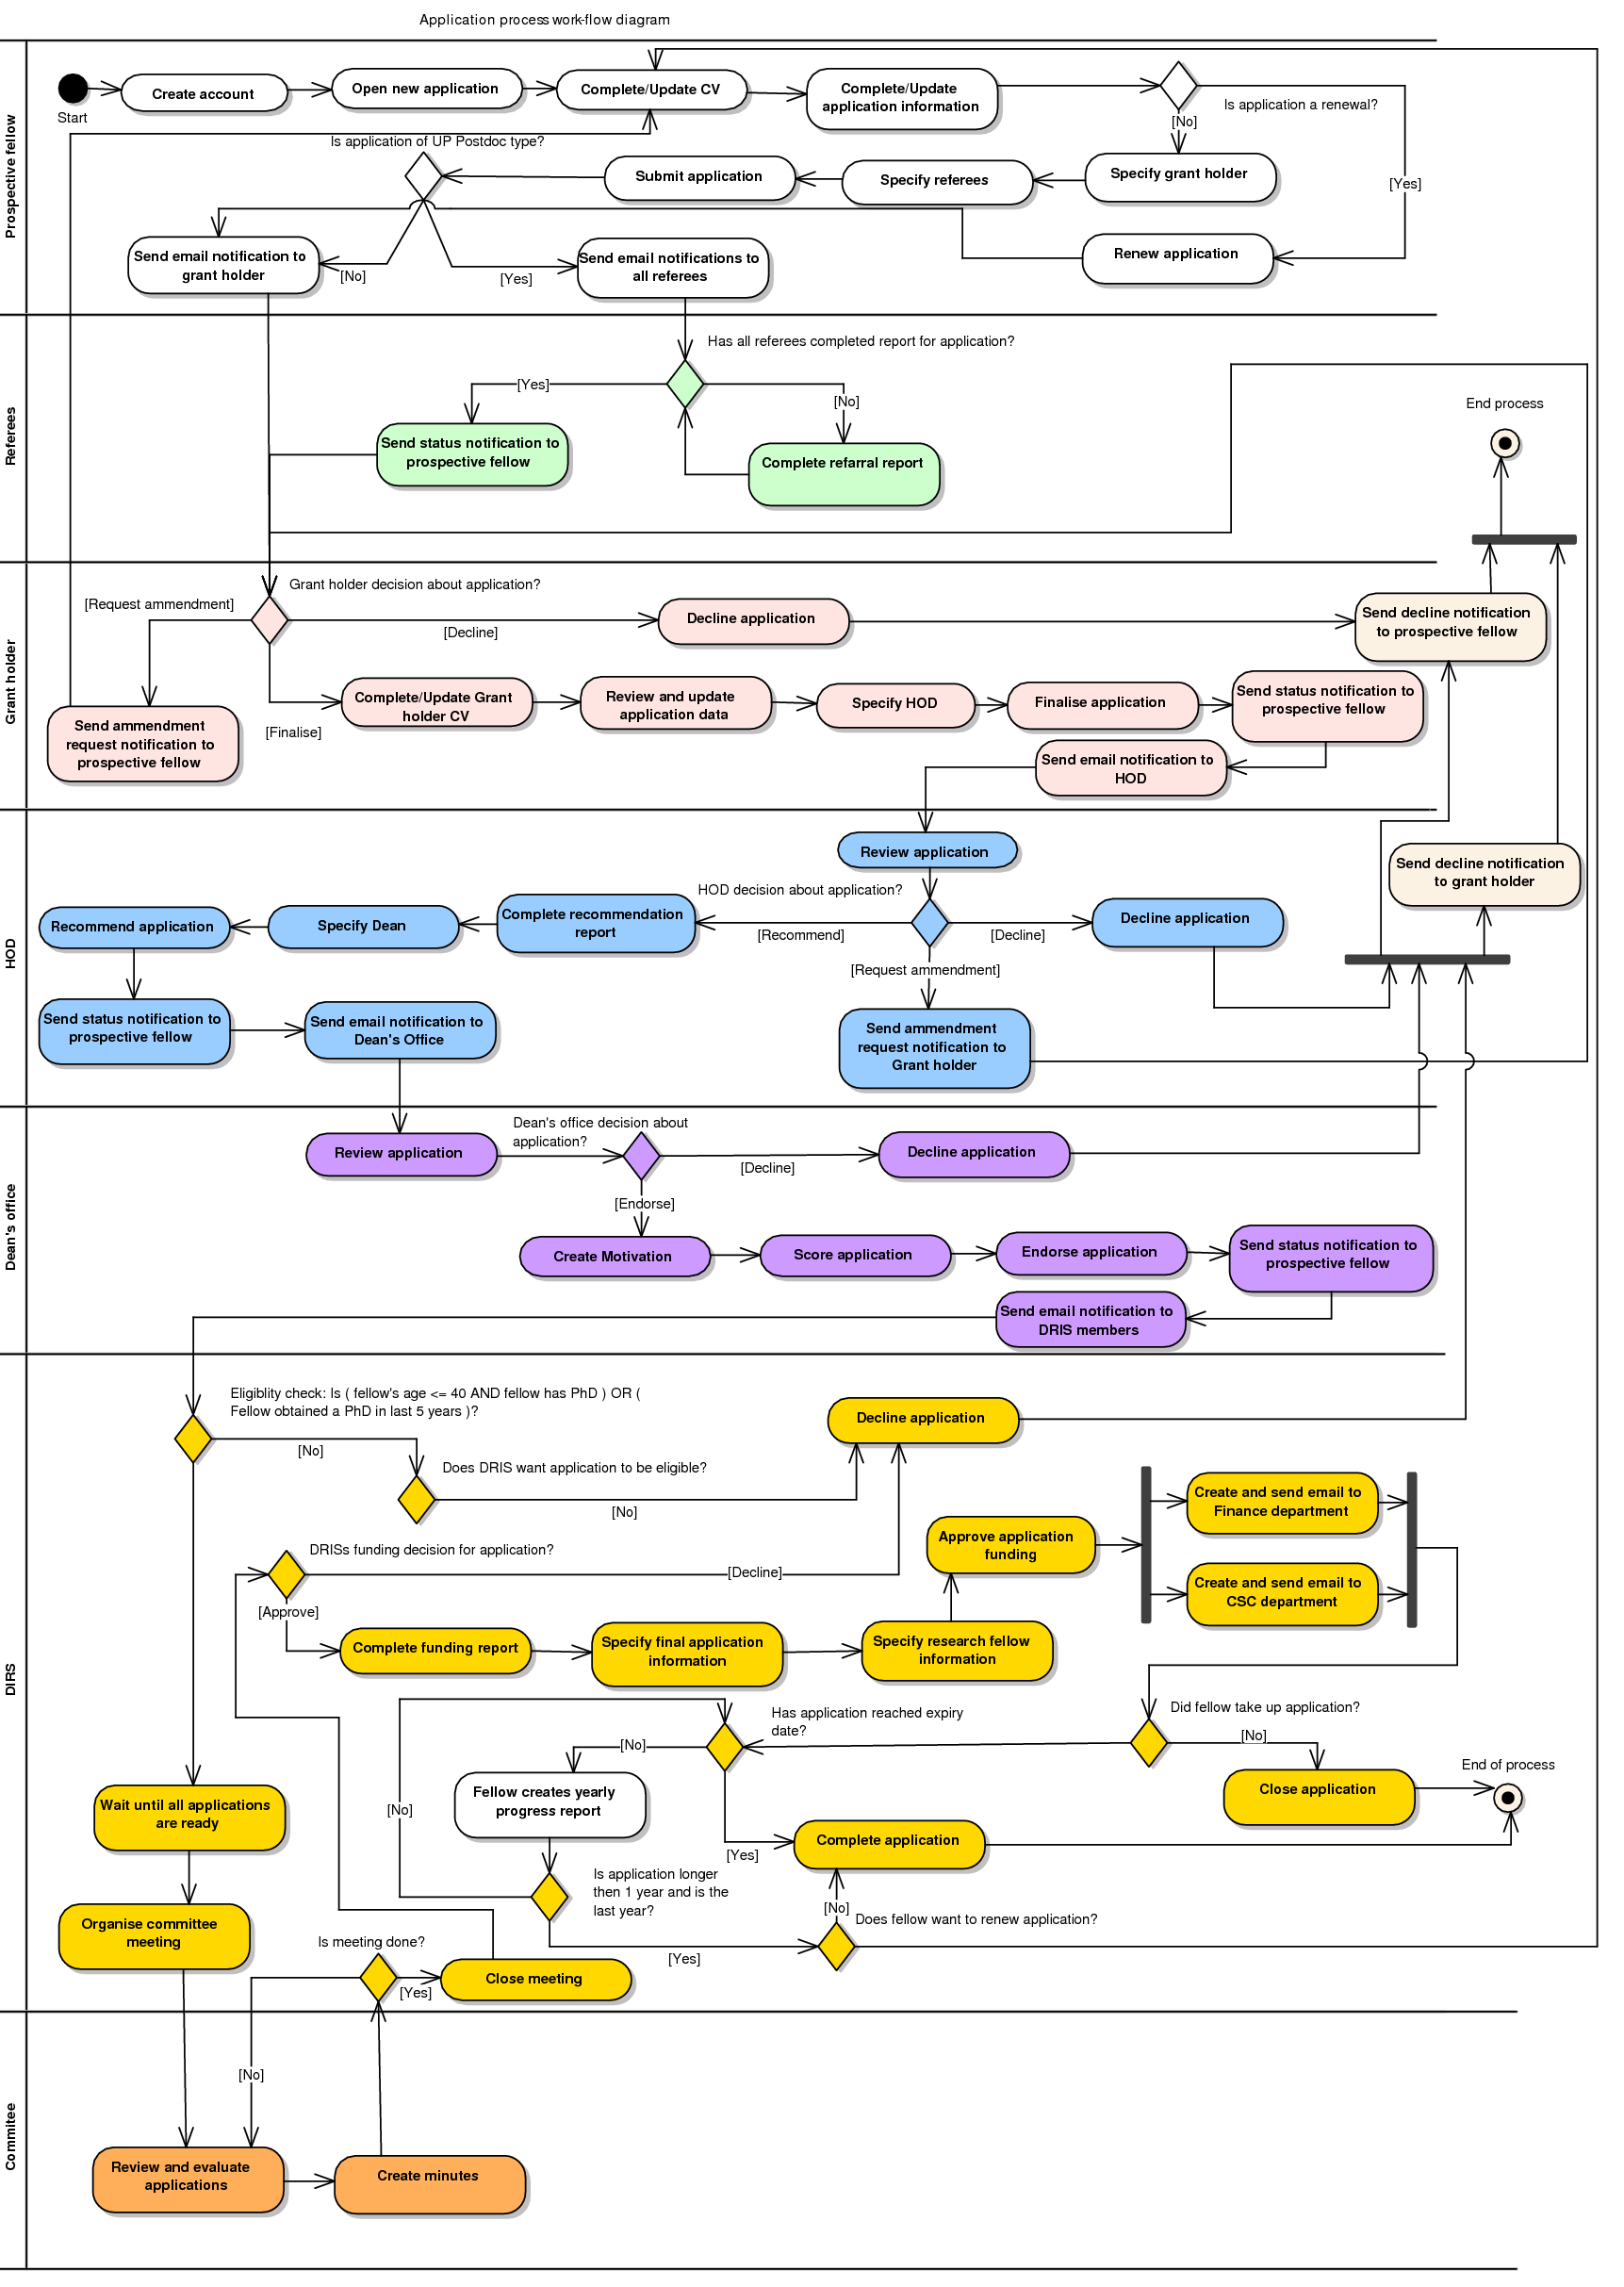
\includegraphics[scale=0.6]{../Images_Docs/Diagrams/Workflow/Workflow model.png}}
\caption{Work-flow diagram of application process}
\end{figure}

\newpage
\subsubsection{Use cases:}
This section shows the use cases for the entire application process. For a more  detailed view of each use cases please refer to the Functional requirements and application design document for the project 

\begin{figure}[H]
\centering	
\framebox{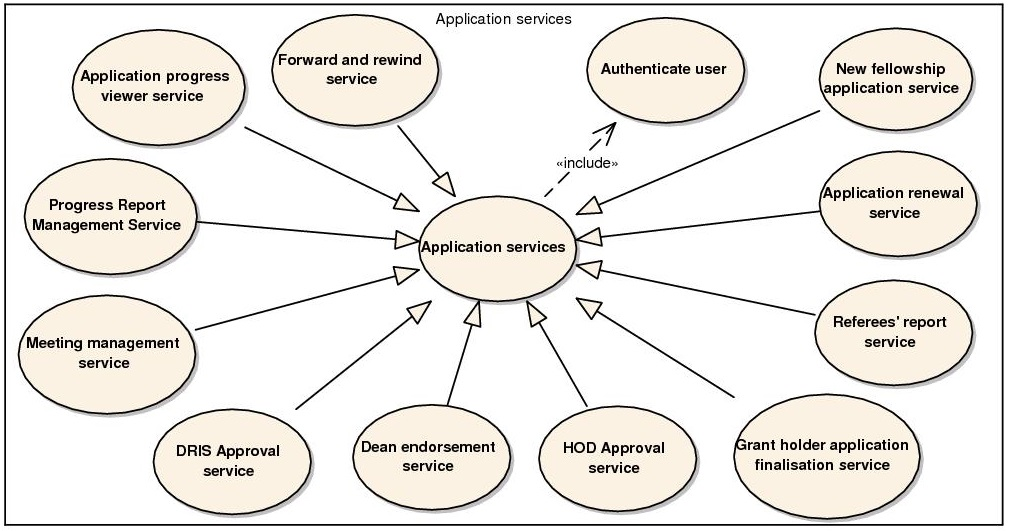
\includegraphics[scale=0.8]{../Images_Docs/Diagrams/Use case diagrams/Application services1.jpg}}
\caption{Use case diagram of Application service}
\end{figure}

\newpage
\vspace{0.2in}
\subsection{Non-application services scope}
This section highlights all the services that aren't part of the application processes but serve other purposes. These services as the name implies can also be used by the system to preform tasks not related to the application processes that help with administration, maintenance of the system and information extraction from system data. Such services include:
\begin{itemize}
	\item Audit-trail services which track critical user actions.
	\item Archival services that manges the backup and archival of data in the data store of system.
	\item User account management services which allows the administration of user accounts.
	\item Notifier services which track outstanding tasks for users.
	\item Location management services which handles the administration of the University's internal academic structure.
	\item Announcement services which help provide a means for system administrators to rely information with users.
	\item Report services which allows for extraction of application and user data in a human readable fashion.
	\item Pre post condition management services which allow system administrators change business rule by altering pre and post conditions of demarcated methods.
	\item Neural network management services which allow the system to host custom neural networks which can be used by system to determine certain data relations. 
\end{itemize}
 
 Some of these services can be used by the application processes to provide additional support to the application work-flow or even enhance it and can also be employed by other services in the system. such services in the scope include:
 \begin{itemize}
 	\item Google scholar services which will provide a means to query google scholar for references and retrieve such search results in a usable manner.
 	\item Notification service which provides a means to send emails and create track-able notifications.
 	\item CV management services which provides the infrastructure for managing user CVs.
 	
\end{itemize} 

\newpage
\subsubsection{Use cases:}
This section shows the use cases for the all the non-application services. For a more detailed view of each use case please refer to the Functional requirements and application design document for the project 

\begin{figure}[H]
\centering	
\framebox{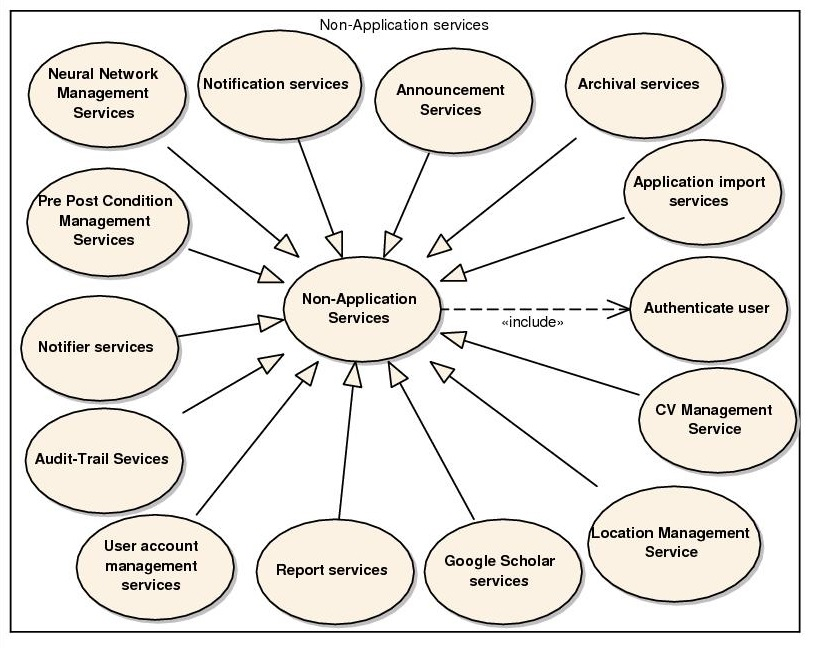
\includegraphics[scale=1]{../Images_Docs/Diagrams/Use case diagrams/Non-Application Services1.jpg}}
\caption{Use case diagram of Non-Application services}
\end{figure}

\vspace{0.2in}
\subsection{Limitations}
\vspace{0.2in}
At the time of writing the project is only limited with regards to the integration with the UP network and the UP's current student and personnel management system. This is due to the IT department of UP only being willing to offer these services or knowledge once the project has been successfully completed. But the system will be developed in such a way to consider the known integration requirements, which at this stage is still very limited. But the fact that the system will provide an API for possible system integration should be able to overcome any problems. 

\subsubsection{Exclusions}
\vspace{0.2in}
Everything not included in this document in terms of scope is considered not in the scope of the project. Though due to the Agile methodology that is employed by the project the scope may be extended or reduced in later iterations if approved by the client.
\\
It should be noted that the client has reduced the scope due to a delay in the development process therefore the Archival services has been backlogged and is kept in the documentation for future implementations.
\vspace{0.2in}

\newpage
\section{Glossary:}
\vspace{0.2in}

\begin{itemize}
\item \textbf{Activity diagram} - A UML diagram that depicts the flow of actions or activities in the process.
\item \textbf{API} - Application Programming Interface
\item \textbf{Application} -Both renewal applications or new fellowship applications are seen as applications by this project.
\item \textbf{CV} - Curriculum Vita
\item \textbf{Domain objects} - Are the objects that are present in the system being modelled.
\item \textbf{EAI} - Enterprise Application Integration
\item \textbf{NRF} - National Research Foundation
\item \textbf{Spreadsheet} - A special type of computer document that is used to represent data in rows and columns.
\item \textbf{GlassFish} - GlassFish is a web server software package that is very flexible and compatible with Java EE applications. 
\item \textbf{HTML} - Hyper Text Mark-up Language
\item \textbf{HTTPS} - Hyper Text Transfer Protocol Secure is a higher level network oriented communication rule set that is highly secure and is used by all web browsers. 
\item \textbf{Java EE} - Java Enterprise Edition
\item \textbf{MySQL} - Is a relational persistence database package that provides all the necessary management tools to run and manage a database server.
\item \textbf{Object-Oriented} - A programming language style that encapsulates everything as an object instance of a particular class of attributes and methods.
\item \textbf{JDBC} - Java Database Connection
\item \textbf{MVC} - Model View Controller
\item \textbf{PDF} - Portable Document Format file
\item \textbf{Peoplesoft} - A management system designed by oracle. 
\item \textbf{Spreadsheet} - A special type of digital document that is used to represent data in rows and columns
\item \textbf{UI} - User Interface
\item \textbf{Use case diagram} - A UML diagram that gives a visual depiction of a service or group of services.
\item \textbf{UML} - Unified modelling language. A commonly used model standard to provide technology neutral models of different aspects of software.
\item \textbf{UP} - University of Pretoria
\item \textbf{Application} - Both a renewal and new fellowship are seen as applications.

\end{itemize}		


\vspace{0.5in}


\end{document}